
%(BEGIN_QUESTION)
% Copyright 2015, Tony R. Kuphaldt, released under the Creative Commons Attribution License (v 1.0)
% This means you may do almost anything with this work of mine, so long as you give me proper credit

One of the most important steps in programming an HMI (Human-Machine Interface) to communication with a PLC is to configure its {\it tagname database}.  This is a list of all data points within the PLC that the HMI must read from and/or write to, as well as any data points within the HMI itself needed for the graphical interface to operate.

Your task is to configure your own HMI panel twice: once to read and write data points for a Koyo CLICK PLC, and again to read and write data points for an Allen-Bradley SLC 500 PLC.  Show your completed tagname database listings (captured screenshots are okay) to the instructor for verification.

\vskip 10pt

{\bf Data points for Koyo CLICK PLC}
\begin{itemize}
\item{} Discrete input {\tt X6} (assign HMI tagname ``Speed\_switch'')
\item{} Discrete output {\tt Y2} (assign HMI tagname ``Alarm\_siren'')
\item{} Counter {\tt C3} current value (assign HMI tagname ``Overspeed\_count'')
\item{} Timer {\tt T5} current value (assign HMI tagname ``Alarm\_duration'')
\end{itemize}

\vskip 10pt

{\bf Data points for Allen-Bradley SLC 500 PLC}
\begin{itemize}
\item{} Discrete input {\tt I:3/5} (assign HMI tagname ``Start\_switch'')
\item{} Discrete output {\tt O:1/2} (assign HMI tagname ``Motor\_contactor'')
\item{} Counter {\tt C5:1} accumulator value (assign HMI tagname ``Start\_count'')
\item{} Timer {\tt T4:0} accumulator value (assign HMI tagname ``Run\_time'')
\end{itemize}

\vskip 10pt

Note that you do not need physical access to any of these PLC types in order to construct the HMI tagname databases for them.  All you need to do is configure the HMI editing software as though the HMI {\it will eventually be} communicating with the appropriate PLC, and then build the database accordingly.


\vskip 20pt \vbox{\hrule \hbox{\strut \vrule{} {\bf Suggestions for Socratic discussion} \vrule} \hrule}

\begin{itemize}
\item{} Your HMI will likely give you options for which type of integer variables to select, 16 bit versus 32 bit, signed versus unsigned.  How do you know what is the appropriate integer size for each PLC application?
\end{itemize}

\underbar{file i04590}
%(END_QUESTION)





%(BEGIN_ANSWER)


%(END_ANSWER)





%(BEGIN_NOTES)

{\bf Tagname database for Koyo CLICK PLC:}

$$\includegraphics[width=15.5cm]{i04590x02.eps}$$

\vskip 20pt

{\bf Tagname database for Allen-Bradley SLC 500 PLC:}

$$\includegraphics[width=15.5cm]{i04590x01.eps}$$

%INDEX% PLC, exploratory question (HMI programming)

%(END_NOTES)


